% Chapter Template

\chapter{Proposed Video Summarization System - Modeling \& Implementation} % Main chapter title

\label{Chapter3} % Change X to a consecutive number; for referencing this chapter elsewhere, use \ref{ChapterX}

\lhead{Chapter 3. \emph{Proposed Video Summarization System - Modeling \& Implementation}} % Change X to a consecutive number; this is for the header on each page - perhaps a shortened title
\makeatletter
\def\BState{\State\hskip-\ALG@thistlm}
\makeatother
%----------------------------------------------------------------------------------------
%	SECTION 1
%----------------------------------------------------------------------------------------

\section{Project Pipeline}

\begin{figure}[ht]
	\centering
		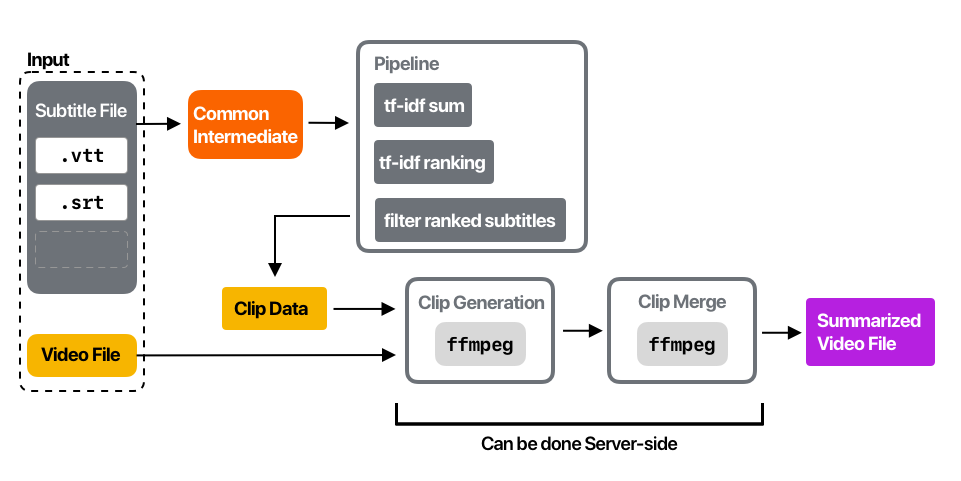
\includegraphics[width=\textwidth, keepaspectratio=true]{Graphic}	
		\caption{Current Pipeline}
		\label{currentpipeline}
\end{figure}

\section{Implementation}

This project creates a video summary taking into account multiple video features. The fact that subtitles are ever-present in videos of today especially in long form videos that warrant summarization, significantly eases this task. Academic videos specifically from portals like NPTEL, Coursera and other MOOC platforms make use of lecture transcriptions in order to facilitate learning which can be easily leveraged in order to enable summarization. 
			
	\subsection{Subtitle Parsing}	
		The current implementation leverages these embedded subtitles by supporting both kinds of popular \verb|.srt| and \verb|.vtt| files extracted from the video. Further, auto-generated YouTube captions can also be utilized for the second module.
			
		The first module takes in the subtitle files, (\verb|.srt| and \verb|.vtt|) and parses them into an intermediate file. This ensures that the text learning module can be run independent of the subtitle format. The intermediate incorporates the subtitle entry length, one-indexed subtitle entry (\verb|.srt| includes indices while \verb|.vtt| lacks indices). The subtitle file reading is chunked to efficiently handle large subtitle files and preventing the whole file from loading onto the memory.
		
		Normally, with long form videos, due to the length of the video, subtitles are often auto-generated by the video hosting provider, e.g. NPTEL videos often utilize auto-generated video subtitles using YouTube due to manual captions being prohibitively hard to implement. These auto-generated video subtitles are generated using a voice to text engine that runs server-side. The subtitle parser can also parse these autogenerated video captions and work on summarization using that, thereby requiring no manual subtitle file input and working off the automatically generated subtitle file.
			
	\subsection{Text Learning}
		Now the second module is invoked which works on the intermediate file generated by the subtitle parser. Common intermediate file is loaded, then punctuation is stripped. Further common English stop words are removed and the subtitle entry string is lemmatized using a \verb|WordNet Lemmatizer|. Next a tf-idf vectorizer is called upon this data which returns the tf-idf matrix.
			
		Summing the tf-idf matrix across columns gives us a column matrix with one cell for each subtitle entry representing the tf-idf sum of the words in the subtitle.
		
		\begin{algorithm}
		\caption{Choosing video clips based on tf-idf sums}
		\label{naivealgo}
		\textbf{Input:} Target length, $t$ and the list of Clip data, $L$ 
		\textbf{Output:} $chosen\_L$, such that $chosen\_L \subseteq L$ and total duration $\leq t$
		\begin{algorithmic}[1]
			\Procedure{GetClips}{}
				\State $t \leftarrow \text{Target clip length}$
				\State $L \leftarrow \text{List of clips}$
				\State $idx \leftarrow 0$
				\State $chosen\_L \leftarrow []$
				\State $L \leftarrow decreasing(L, L['tf\_idf'])$	 \Comment{Sort in decreasing order based on tf-idf values}
				\BState start:
				\If {$t < 0$} 
					\State \Return \textit{chosen\_L}
					\State \textbf{stop}
				\EndIf
				\State $t \leftarrow t - L[\textit{idx}].duration$
				\State $chosen\_L.append(L[idx])$
				\State $idx \leftarrow idx + 1$
				\State \textbf{goto} \textit{start}
			\EndProcedure
		\end{algorithmic}
	\end{algorithm}
			
		Since, the parser module also returns the duration of a subtitle, arranging it in descending order and summing up the durations till it exceeds the required length gives the subtitle entries to include in the final output video (as shown in Algorithm~\ref{naivealgo}).
	    
	    \begin{algorithm}
		\textbf{Input:} Naively chosen clips, $chosen\_L$ and the Flexibility Parameter, $F$ 
		
		\textbf{Output:} A flexibly extended list of clips, $Flex\_L$, such that $chosen\_L \subseteq Flex\_L \subseteq L$.
		\caption{Extend naively chosen clips with clips selected using Flexibility Parameter}
		\label{FParamAlg}
		\begin{algorithmic}[1]
			\Procedure{ExtendSelection}{}
				\State $selected \leftarrow []$		
				\State $idx \leftarrow 0$
				\State $len\_selected \leftarrow len(chosen\_L)$
				\BState indexLoop:
					\If{$L[idx]$ in $chosen\_L$} \State $selected.append(idx)$
					\EndIf
					\State $idx \leftarrow idx + 1$
					\If{$idx < len(chosen\_L)$} \State \textbf{goto} \textit{indexLoop}
					\Else \State \textbf{goto} \textit{main}
					\EndIf
				\BState main:
					\State $idx \leftarrow 0$
					\State $Flex\_L \leftarrow selected$
					\State \textbf{goto} \textit{loop}
					\BState loop:
						\If {$selected[ idx + 1] - selected[idx]\leq F~\&\&~selected[idx+1] - selected[idx] > 1$}
							\State $Flex\_L.append([selected[idx]+1 \hdots selected[idx + 1])$
						\EndIf
						\If{$idx \leq len(selected) - 2$}
							\State $idx \leftarrow idx + 1$
						\Else
							\State \textbf{stop}
						\EndIf
			\EndProcedure
		\end{algorithmic}
	\end{algorithm}
	    
    	\subsubsection{Flexibility Parameter}
    		Now the concept of a flexibility parameter is introduced. This is depicted in the Figure~\ref{flexparam}, where the green entries indicate the initially selected subtitle entries based on the tf-idf sum ranking. 

            The process of selecting this Flexibility Parameter is described in Algorithm~\ref{FParamAlg}.
            
    		Based on the value of the flexibility parameter, say \(N\), selected subtitle entries with \(\leq N\) unselected entries in between are also selected.
    				
    		Setting the parameter to zero generates a summary that's as close as possible to the required length. Whereas, setting the parameter to a large value will include the whole video.
    				
    				\begin{figure}[ht]
    				\centering
    					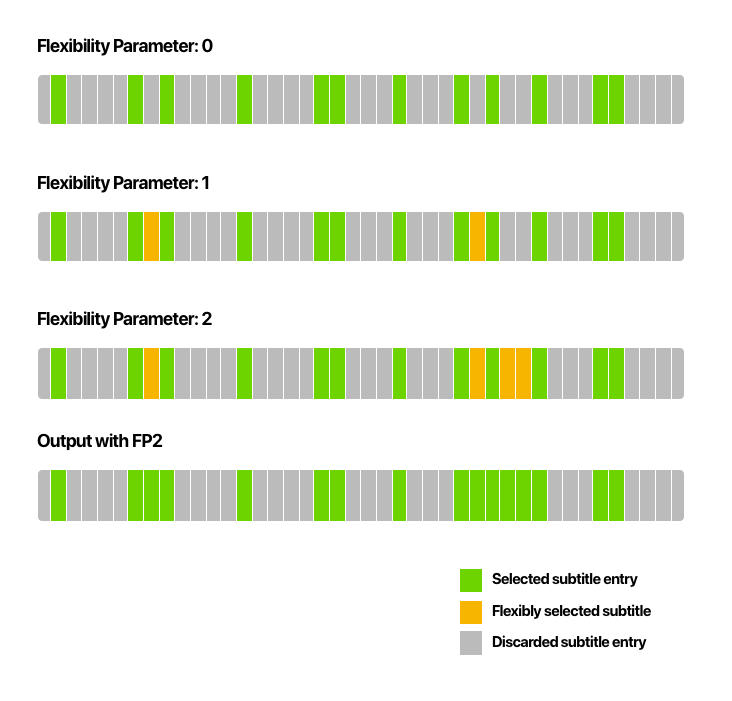
\includegraphics[width=0.5\textwidth, keepaspectratio=true]{Flexibility}	
    					\caption{Flexibility Parameter}
    					\label{flexparam}
    				\end{figure}
    				
    				\begin{mdframed}
    					\textbf{\underline{Need}}
    					
    						The concept of flexibility parameter tackles the fundamental idea that if two subtitle entries close by are important then the subtitles between them are important enough to be included in the summary.
    						
    						This also ensures that the final output is smoother and is not jarring to view. As a result of the flexibility parameter, the final video output becomes longer than the required length.
    				\end{mdframed}
    			This module creates another intermediate file with the start time, end time and the index of the clips to cut and join to create the summary. 
		
		\subsection{Clip and Summary Creation}	
			Now the final module takes in the intermediate clip data and parses it. It takes in the time stamps and rounds it. The subtitle entries in the original subtitle file have exact times (down to microseconds) to start showing subtitles and to stop showing the subtitles. This is removed when the start times are floored down and the stop times are ceiled up. 
			
			\begin{algorithm}
		\caption{Algorithm to get contiguous sequences of clips}
		\label{contiguous}
		\textbf{Input:} Indices of the subtitle file chosen, $chosen$
		\textbf{Output:} A list of lists $sets\_of\_clips$, consisting of contiguous sequences of clip data.
		
		\begin{algorithmic}[1]
			\Procedure{ContiguousClips}{}
				\State $idx \leftarrow 0$
				\State $sets\_of\_clips \leftarrow []$
				\State $temp \leftarrow []$
				\BState loop:
					\If{$chosen[idx]~\textbf{not in}~temp$}
						\State $temp.append(chosen[idx])$
					\EndIf
					
					\If {$chosen[idx+1]-chosen[idx] == 1$}
            			\State $temp.append(chosen[idx+1])$
            			\State \textbf{continue}
			        \Else
			            \State $sets\_of\_clips.append(temp)$
			            \State $temp \leftarrow []$
					\EndIf
					\If{$idx \leq len(selected) - 2$}
							\State $idx \leftarrow idx + 1$
						\Else
						    \State \textbf{return} \textit{sets\_of\_clips}
							\State \textbf{stop}
						\EndIf
			\EndProcedure
		\end{algorithmic}
	\end{algorithm}
			
			Further, contiguous sequences of clips are identified and taken together in order the determine the start and the end time of the final clip using Algorithm~\ref{contiguous}. Thus, if say the subtitle entries with indices $1,2,3,4$ are selected, then this ensures that the start time of 1 and the end time of 4 are taken for the purposes of cropping the video.
			
			Next the multiprocessing module calls \verb|ffmpeg| running parallel on the processor of the computer. Finally the created subclips are merged together, again using \verb|ffmpeg| to create the output. \verb|ffmpeg| uses hardware acceleration to encode video streams (For example, h264\_videotoolbox and h265\_videotoolbox are Apple's GPU access API on macOS and \verb|nvenc| for nVidia GPUs).
			
			\begin{mdframed}
				\textbf{\underline{Advantages}}\\
					Since the clip creation and summary generation is running independent as long as the video and the subclip intermediate is available, the initial generation can be done on-device and then the heavy work can be run completely server side leveraging large parallel processing power.
			\end{mdframed}
	
	\subsection{Audio Processing}
	    The audio processing pipeline consists primarily of the following steps:
	    
	    \begin{enumerate}
	        \item \textbf{Audio Extraction:}
	            This step involves extracting the audio waveform file from the input video, into it's constitutent audio file and video file.
	        \item \textbf{Audio Pre-processing:}
	            This step is implemented using the \texttt{ffmpeg} library and selectively encoding the audio track to a separate \texttt{.wav} file in order to enable processing.
            \item \textbf{Audio Feature Extraction:}
                This process involves extracting features from the exported audio file. Explored feature extraction techniques include:
                \begin{itemize}
                    \item \textbf{MFCC:} Mel Frequency Cepstral Coefficient are Coefficients of the Mel-frequency spectrum that resemble how a human hears audio, with high emphasis on lower frequencies and lower emphasis on high frequencies.
                \end{itemize}
            \item \textbf{Learning from Audio:} This process involves mining information from the extracted audio file. Multiple kinds of information can be extracted from the audio track.
                \begin{itemize}
                    \item Emotion Detection and Energy Detection
                    \item Voice activity detection
                \end{itemize}
            Work is being done to determine which will serve most suitable to the purposes of enhancing video sumamrization with additional cues.
	    \end{enumerate}